\PassOptionsToPackage{unicode=true}{hyperref} % options for packages loaded elsewhere
\PassOptionsToPackage{hyphens}{url}
%
\documentclass[]{book}
\usepackage{lmodern}
\usepackage{amssymb,amsmath}
\usepackage{ifxetex,ifluatex}
\usepackage{fixltx2e} % provides \textsubscript
\ifnum 0\ifxetex 1\fi\ifluatex 1\fi=0 % if pdftex
  \usepackage[T1]{fontenc}
  \usepackage[utf8]{inputenc}
  \usepackage{textcomp} % provides euro and other symbols
\else % if luatex or xelatex
  \usepackage{unicode-math}
  \defaultfontfeatures{Ligatures=TeX,Scale=MatchLowercase}
\fi
% use upquote if available, for straight quotes in verbatim environments
\IfFileExists{upquote.sty}{\usepackage{upquote}}{}
% use microtype if available
\IfFileExists{microtype.sty}{%
\usepackage[]{microtype}
\UseMicrotypeSet[protrusion]{basicmath} % disable protrusion for tt fonts
}{}
\IfFileExists{parskip.sty}{%
\usepackage{parskip}
}{% else
\setlength{\parindent}{0pt}
\setlength{\parskip}{6pt plus 2pt minus 1pt}
}
\usepackage{hyperref}
\hypersetup{
            pdftitle={Notes for STAT 5413 - Spatial Statistics},
            pdfauthor={John Tipton},
            pdfborder={0 0 0},
            breaklinks=true}
\urlstyle{same}  % don't use monospace font for urls
\usepackage{color}
\usepackage{fancyvrb}
\newcommand{\VerbBar}{|}
\newcommand{\VERB}{\Verb[commandchars=\\\{\}]}
\DefineVerbatimEnvironment{Highlighting}{Verbatim}{commandchars=\\\{\}}
% Add ',fontsize=\small' for more characters per line
\usepackage{framed}
\definecolor{shadecolor}{RGB}{248,248,248}
\newenvironment{Shaded}{\begin{snugshade}}{\end{snugshade}}
\newcommand{\AlertTok}[1]{\textcolor[rgb]{0.94,0.16,0.16}{#1}}
\newcommand{\AnnotationTok}[1]{\textcolor[rgb]{0.56,0.35,0.01}{\textbf{\textit{#1}}}}
\newcommand{\AttributeTok}[1]{\textcolor[rgb]{0.77,0.63,0.00}{#1}}
\newcommand{\BaseNTok}[1]{\textcolor[rgb]{0.00,0.00,0.81}{#1}}
\newcommand{\BuiltInTok}[1]{#1}
\newcommand{\CharTok}[1]{\textcolor[rgb]{0.31,0.60,0.02}{#1}}
\newcommand{\CommentTok}[1]{\textcolor[rgb]{0.56,0.35,0.01}{\textit{#1}}}
\newcommand{\CommentVarTok}[1]{\textcolor[rgb]{0.56,0.35,0.01}{\textbf{\textit{#1}}}}
\newcommand{\ConstantTok}[1]{\textcolor[rgb]{0.00,0.00,0.00}{#1}}
\newcommand{\ControlFlowTok}[1]{\textcolor[rgb]{0.13,0.29,0.53}{\textbf{#1}}}
\newcommand{\DataTypeTok}[1]{\textcolor[rgb]{0.13,0.29,0.53}{#1}}
\newcommand{\DecValTok}[1]{\textcolor[rgb]{0.00,0.00,0.81}{#1}}
\newcommand{\DocumentationTok}[1]{\textcolor[rgb]{0.56,0.35,0.01}{\textbf{\textit{#1}}}}
\newcommand{\ErrorTok}[1]{\textcolor[rgb]{0.64,0.00,0.00}{\textbf{#1}}}
\newcommand{\ExtensionTok}[1]{#1}
\newcommand{\FloatTok}[1]{\textcolor[rgb]{0.00,0.00,0.81}{#1}}
\newcommand{\FunctionTok}[1]{\textcolor[rgb]{0.00,0.00,0.00}{#1}}
\newcommand{\ImportTok}[1]{#1}
\newcommand{\InformationTok}[1]{\textcolor[rgb]{0.56,0.35,0.01}{\textbf{\textit{#1}}}}
\newcommand{\KeywordTok}[1]{\textcolor[rgb]{0.13,0.29,0.53}{\textbf{#1}}}
\newcommand{\NormalTok}[1]{#1}
\newcommand{\OperatorTok}[1]{\textcolor[rgb]{0.81,0.36,0.00}{\textbf{#1}}}
\newcommand{\OtherTok}[1]{\textcolor[rgb]{0.56,0.35,0.01}{#1}}
\newcommand{\PreprocessorTok}[1]{\textcolor[rgb]{0.56,0.35,0.01}{\textit{#1}}}
\newcommand{\RegionMarkerTok}[1]{#1}
\newcommand{\SpecialCharTok}[1]{\textcolor[rgb]{0.00,0.00,0.00}{#1}}
\newcommand{\SpecialStringTok}[1]{\textcolor[rgb]{0.31,0.60,0.02}{#1}}
\newcommand{\StringTok}[1]{\textcolor[rgb]{0.31,0.60,0.02}{#1}}
\newcommand{\VariableTok}[1]{\textcolor[rgb]{0.00,0.00,0.00}{#1}}
\newcommand{\VerbatimStringTok}[1]{\textcolor[rgb]{0.31,0.60,0.02}{#1}}
\newcommand{\WarningTok}[1]{\textcolor[rgb]{0.56,0.35,0.01}{\textbf{\textit{#1}}}}
\usepackage{longtable,booktabs}
% Fix footnotes in tables (requires footnote package)
\IfFileExists{footnote.sty}{\usepackage{footnote}\makesavenoteenv{longtable}}{}
\usepackage{graphicx,grffile}
\makeatletter
\def\maxwidth{\ifdim\Gin@nat@width>\linewidth\linewidth\else\Gin@nat@width\fi}
\def\maxheight{\ifdim\Gin@nat@height>\textheight\textheight\else\Gin@nat@height\fi}
\makeatother
% Scale images if necessary, so that they will not overflow the page
% margins by default, and it is still possible to overwrite the defaults
% using explicit options in \includegraphics[width, height, ...]{}
\setkeys{Gin}{width=\maxwidth,height=\maxheight,keepaspectratio}
\setlength{\emergencystretch}{3em}  % prevent overfull lines
\providecommand{\tightlist}{%
  \setlength{\itemsep}{0pt}\setlength{\parskip}{0pt}}
\setcounter{secnumdepth}{5}
% Redefines (sub)paragraphs to behave more like sections
\ifx\paragraph\undefined\else
\let\oldparagraph\paragraph
\renewcommand{\paragraph}[1]{\oldparagraph{#1}\mbox{}}
\fi
\ifx\subparagraph\undefined\else
\let\oldsubparagraph\subparagraph
\renewcommand{\subparagraph}[1]{\oldsubparagraph{#1}\mbox{}}
\fi

% set default figure placement to htbp
\makeatletter
\def\fps@figure{htbp}
\makeatother

\usepackage{booktabs}
\usepackage{xcolor}
\definecolor{plum}{rgb}{0.56, 0.27, 0.52}
\usepackage[]{natbib}
\bibliographystyle{apalike}

\title{Notes for STAT 5413 - Spatial Statistics}
\author{John Tipton}
\date{Fall 2020 Semester. Last Modified: 2020-01-13}

\begin{document}
\maketitle

{
\setcounter{tocdepth}{1}
\tableofcontents
}
\hypertarget{stat-5413}{%
\chapter{STAT 5413}\label{stat-5413}}

These are the lecture notes for STAT 5413 Fall 2020.

\hypertarget{day-1}{%
\chapter{Day 1}\label{day-1}}

\begin{Shaded}
\begin{Highlighting}[]
\KeywordTok{library}\NormalTok{(tidyverse)}
\end{Highlighting}
\end{Shaded}

\hypertarget{notation}{%
\section{Notation}\label{notation}}

The dimensions of different mathematical objects are very important for the study of spatial statistics. To communicate this, we use the following notation. A scalar random variable is represented by a lowercase alphanumeric letter (\(x\), \(y\), \(z\), etc.), a vector random variable is respresented by a bold lowercase alphanumeric letter (\(\mathbf{x}\), \(\mathbf{y}\), \(\mathbf{z}\), etc.), and a matrix random variable is respresented by a bold uppercase alphanumeric letter (\(\mathbf{X}\), \(\mathbf{Y}\), \(\mathbf{Z}\), etc.). We use a similar notation for parameters as well where scalar parameters are represented by a lowercase Greek letter (\(\mu\), \(\alpha\), \(\beta\), etc.), a vector parameter is respresented by a bold lowercase Greek letter (\(\boldsymbol{\mu}\), \(\boldsymbol{\alpha}\), \(\boldsymbol{\beta}\), etc.), and a matrix random variable is respresented by a bold uppercase Greek letter (\(\boldsymbol{\Sigma}\), \(\boldsymbol{\Psi}\), \(\boldsymbol{\Gamma}\), etc.).

\hypertarget{probability-distributions}{%
\section{Probability Distributions}\label{probability-distributions}}

We also need notation to explain probability distributions. We use the notation \([y]\) to denote the probability density function \(p(y)\) of the random variable \(y\) and \([y|x]\) to denote the probability density function \(p(y|x)\) of \(y\) given \(x\). For example, if \(y\) is a Gaussian random variable with mean \(\mu\) and standard deviation \(\sigma\) we write

\begin{align*}
[y | \mu, \sigma] & = \frac{1}{\sqrt{2 \pi \sigma^2}} \exp \left\{-\frac{1}{2 \sigma^2} (y - \mu)^2 \right\}.
\end{align*}

We can also denote that \(y\) has a Gaussian (normal) distribution given mean \(\mu\) and variance \(\sigma^2\) using the \(\sim\) notation

\begin{align*}
y | \mu, \sigma & \sim \operatorname{N}(\mu, \sigma^2).
\end{align*}

\hypertarget{example-linear-regression}{%
\subsection{Example: linear regression}\label{example-linear-regression}}

\begin{align*}
\left[y_i | \boldsymbol{\theta} \right] & \sim \operatorname{N}(X_i \beta, \sigma^2) \\
\boldsymbol{\theta} & = (\beta, \sigma^2)
\end{align*}

\begin{Shaded}
\begin{Highlighting}[]
\CommentTok{## Sample data}
\KeywordTok{set.seed}\NormalTok{(}\DecValTok{404}\NormalTok{)}
\NormalTok{dat <-}\StringTok{ }\KeywordTok{data.frame}\NormalTok{(}\DataTypeTok{x=}\NormalTok{(}\DataTypeTok{x=}\KeywordTok{runif}\NormalTok{(}\DecValTok{200}\NormalTok{, }\DecValTok{0}\NormalTok{, }\DecValTok{50}\NormalTok{)),}
                  \DataTypeTok{y=}\KeywordTok{rnorm}\NormalTok{(}\DecValTok{200}\NormalTok{, }\DecValTok{10} \OperatorTok{*}\StringTok{ }\NormalTok{x, }\DecValTok{100}\NormalTok{))}

\CommentTok{## breaks: where you want to compute densities}
\NormalTok{breaks <-}\StringTok{ }\KeywordTok{seq}\NormalTok{(}\DecValTok{0}\NormalTok{, }\KeywordTok{max}\NormalTok{(dat}\OperatorTok{$}\NormalTok{x), }\DataTypeTok{len=}\DecValTok{7}\NormalTok{)[}\OperatorTok{-}\KeywordTok{c}\NormalTok{(}\DecValTok{1}\NormalTok{, }\DecValTok{7}\NormalTok{)]}
\NormalTok{dat}\OperatorTok{$}\NormalTok{section <-}\StringTok{ }\KeywordTok{cut}\NormalTok{(dat}\OperatorTok{$}\NormalTok{x, breaks)}

\CommentTok{## Get the residuals}
\NormalTok{dat}\OperatorTok{$}\NormalTok{res <-}\StringTok{ }\KeywordTok{residuals}\NormalTok{(}\KeywordTok{lm}\NormalTok{(y }\OperatorTok{~}\StringTok{ }\NormalTok{x, }\DataTypeTok{data=}\NormalTok{dat))}

\CommentTok{## Compute densities for each section, and flip the axes, and add means of sections}
\CommentTok{## Note: the densities need to be scaled in relation to the section size (2000 here)}
\NormalTok{ys <-}\StringTok{ }\KeywordTok{seq}\NormalTok{(}\OperatorTok{-}\DecValTok{300}\NormalTok{, }\DecValTok{300}\NormalTok{, }\DataTypeTok{length =} \DecValTok{50}\NormalTok{)}
\NormalTok{xs <-}\StringTok{ }\KeywordTok{rep}\NormalTok{(breaks, }\DataTypeTok{each =} \DecValTok{50}\NormalTok{) }\OperatorTok{+}\StringTok{ }\DecValTok{1000} \OperatorTok{*}\StringTok{ }\KeywordTok{dnorm}\NormalTok{(ys, }\DecValTok{0}\NormalTok{, }\DecValTok{100}\NormalTok{)}
\NormalTok{res <-}\StringTok{ }\KeywordTok{matrix}\NormalTok{(}\DecValTok{0}\NormalTok{, }\DecValTok{50}\NormalTok{, }\DecValTok{5}\NormalTok{)}
\ControlFlowTok{for}\NormalTok{ (i }\ControlFlowTok{in} \DecValTok{1}\OperatorTok{:}\DecValTok{5}\NormalTok{) \{}
\NormalTok{  res[, i] <-}\StringTok{ }\DecValTok{10} \OperatorTok{*}\StringTok{ }\NormalTok{breaks[i] }\OperatorTok{+}\StringTok{ }\NormalTok{ys }
\NormalTok{\}}
\NormalTok{dens <-}\StringTok{ }\KeywordTok{data.frame}\NormalTok{(}\DataTypeTok{x =}\NormalTok{ xs, }\DataTypeTok{y=}\KeywordTok{c}\NormalTok{(res), }
                   \DataTypeTok{grouping =} \KeywordTok{cut}\NormalTok{(xs, breaks))}
\KeywordTok{ggplot}\NormalTok{(dat, }\KeywordTok{aes}\NormalTok{(x, y)) }\OperatorTok{+}
\StringTok{  }\KeywordTok{geom_point}\NormalTok{(}\DataTypeTok{size =} \DecValTok{2}\NormalTok{) }\OperatorTok{+}
\StringTok{  }\KeywordTok{geom_smooth}\NormalTok{(}\DataTypeTok{method=}\StringTok{"lm"}\NormalTok{, }\DataTypeTok{fill=}\OtherTok{NA}\NormalTok{, }\DataTypeTok{lwd=}\DecValTok{2}\NormalTok{, }\DataTypeTok{se =} \OtherTok{FALSE}\NormalTok{) }\OperatorTok{+}
\StringTok{  }\KeywordTok{geom_path}\NormalTok{(}\DataTypeTok{data=}\NormalTok{dens, }\KeywordTok{aes}\NormalTok{(x, y, }\DataTypeTok{group =}\NormalTok{ grouping), }
            \DataTypeTok{color=}\StringTok{"salmon"}\NormalTok{, }\DataTypeTok{lwd=}\DecValTok{2}\NormalTok{) }\OperatorTok{+}
\StringTok{  }\KeywordTok{theme_bw}\NormalTok{() }\OperatorTok{+}
\StringTok{  }\KeywordTok{geom_vline}\NormalTok{(}\DataTypeTok{xintercept=}\NormalTok{breaks, }\DataTypeTok{lty=}\DecValTok{2}\NormalTok{)}
\end{Highlighting}
\end{Shaded}

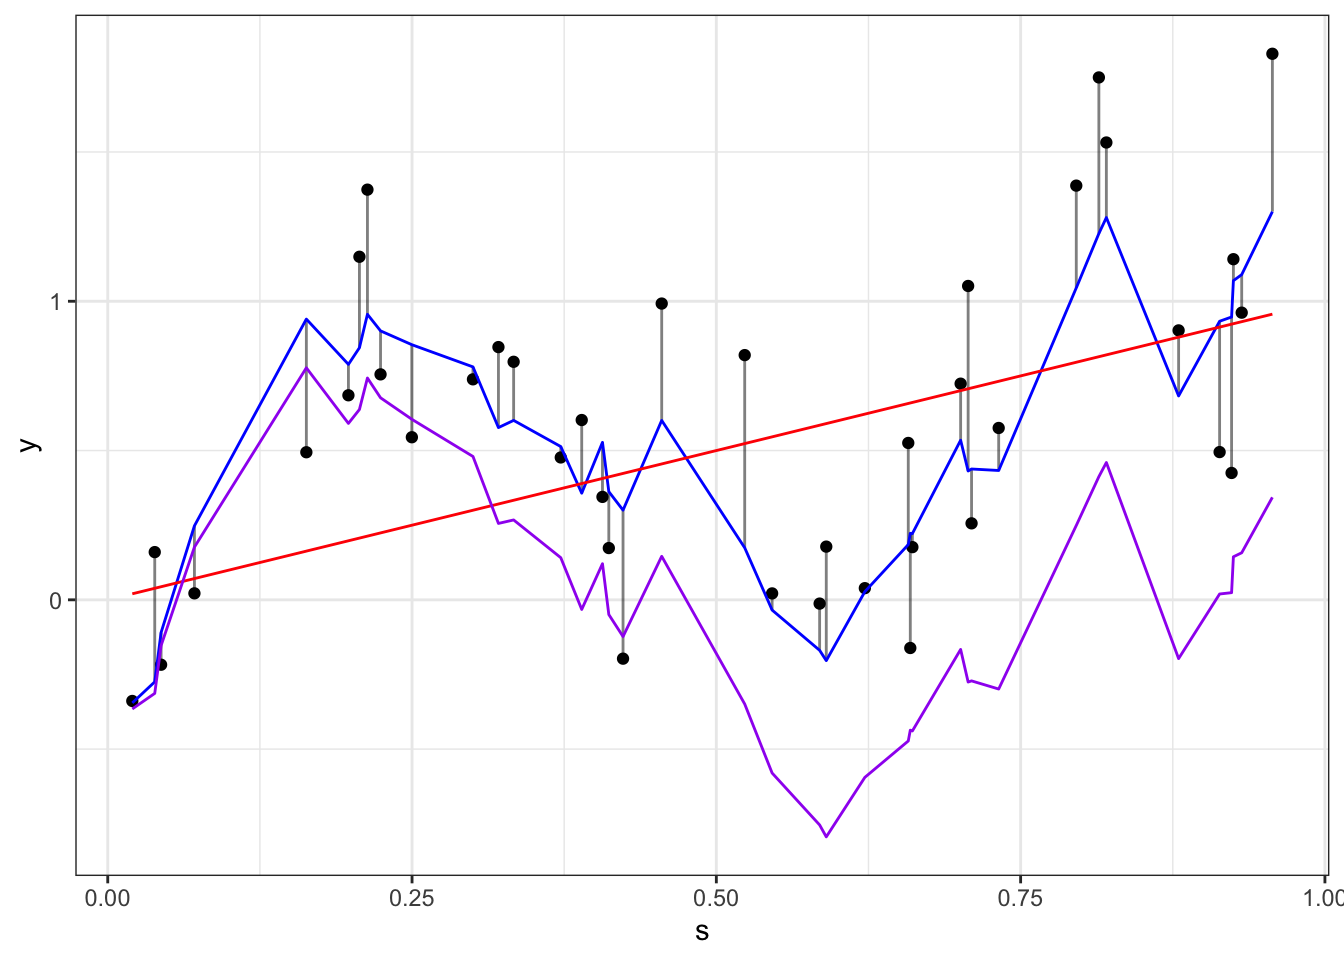
\includegraphics[width=0.8\linewidth]{STAT-5413_files/figure-latex/unnamed-chunk-2-1}

\hypertarget{hierarchical-modeling}{%
\section{Hierarchical modeling}\label{hierarchical-modeling}}

\begin{itemize}
\item
  Follow \citet{berliner1996hierarchical} framework for hierarchical probability models
\item
  Model encodes our understanding of the scientific process of interest
\item
  Model accounts for as much uncertainty as possible
\item
  Model results in a probability distribution

  \begin{itemize}
  \tightlist
  \item
    Note: nature may be deterministic -- often probabilistic models outperform physical models.
  \item
    Example: model individual rain drops vs.~probability/intensity of rain
  \end{itemize}
\item
  Update model with data
\item
  Use the model to generate parameter estimates given data
\end{itemize}

\hypertarget{bayesian-hierarchical-models-bhms}{%
\subsection{Bayesian Hierarchical models (BHMs)}\label{bayesian-hierarchical-models-bhms}}

\begin{itemize}
\item
  Break the model into components:

  \begin{itemize}
  \item
    { Data Model. }
  \item
    { Process Model. }
  \item
    { Parameter Model. }
  \end{itemize}
\item
  Combined, the { data model, } the { process model, } and the { parameter model } define a { posterior distribution. }
\end{itemize}

\begin{align*}
\color{cyan}{[\mathbf{z}, \boldsymbol{\theta}_D, \boldsymbol{\theta}_P | \mathbf{y}]} & \propto
\color{red}{[\mathbf{y} | \boldsymbol{\theta}_D, \mathbf{z}]}  \color{blue}{[\mathbf{z} | \boldsymbol{\theta}_P]} \color{orange}{[\boldsymbol{\theta}_D] [\boldsymbol{\theta}_P]}
\end{align*}

\hypertarget{empirical-hierarchical-models-ehms}{%
\subsection{Empirical Hierarchical models (EHMs)}\label{empirical-hierarchical-models-ehms}}

\begin{itemize}
\item
  Break the model into components:

  \begin{itemize}
  \item
    { Data Model. }
  \item
    { Process Model. }
  \item
    { Parameter estimates } (fixed values) are substituted before fitting the model
  \end{itemize}
\item
  Combined, the { data model and } the { process model } define a { predictive distribution. } Thus, numerical evaluation of the { predictive distribution } is typically required to estimate unceratinty (bootstrap, MLE asymptotics)

  \begin{itemize}
  \tightlist
  \item
    Note: the predictive distribution is not a {posterior distribution} because the normalizing constant is not known
  \end{itemize}
\end{itemize}

\begin{align*}
\color{plum}{[\mathbf{z} | \mathbf{y}]} & \propto
\color{red}{[\mathbf{y} | \boldsymbol{\theta}_D, \mathbf{z}]}  \color{blue}{[\mathbf{z} | \boldsymbol{\theta}_P]}
\end{align*}

\hypertarget{data-model}{%
\subsection{Data Model}\label{data-model}}

\begin{align*}
\color{red}{[\mathbf{y} | \boldsymbol{\theta}_D, \mathbf{z}]}
\end{align*}

\begin{itemize}
\item
  Describes how the data are collected and observed.
\item
  Account for measurement process and uncertainty.
\item
  Model the data in the manner in which they were collected.
\item
  Data \(\mathbf{y}\).

  \begin{itemize}
  \item
    Noisy.
  \item
    Expensive.
  \item
    Not what you want to make inference on.
  \end{itemize}
\item
  Latent variables \(\mathbf{z}\).

  \begin{itemize}
  \item
    Think of \(\mathbf{z}\) as the ideal data.
  \item
    No measurement error - the exact quantity you want to observe but can't.
  \end{itemize}
\item
  Data model parameters \(\boldsymbol{\theta}_D\).
\end{itemize}

\hypertarget{process-model}{%
\subsection{Process Model}\label{process-model}}

\begin{align*}
\color{blue}{[\mathbf{z} | \boldsymbol{\theta}_P]} 
\end{align*}

\begin{itemize}
\item
  \textbf{Where the science happens!}
\item
  Latent process \(\mathbf{z}\) is modeled.
\item
  Can be dynamic in space and/or time
\item
  Process parameters \(\boldsymbol{\theta}_P\).
\item
  Virtually all interesting scientific questions can be made with inference about \(\mathbf{z}\)
\end{itemize}

\hypertarget{parameter-prior-model-bmhs-only}{%
\subsection{Parameter (Prior) Model (BMHs only)}\label{parameter-prior-model-bmhs-only}}

\begin{align*}
\color{orange}{[\boldsymbol{\theta}_D] [\boldsymbol{\theta}_P]}
\end{align*}

\begin{itemize}
\item
  Probability distributions define ``reasonable'' ranges for parameters.
\item
  Parameter models are useful for a variety of problems:

  \begin{itemize}
  \item
    Choosing important variables.
  \item
    Preventing over-fitting (regularization).
  \item
    ``Pooling'' estimates across categories.
  \end{itemize}
\end{itemize}

\hypertarget{posterior-distribution}{%
\subsection{Posterior Distribution}\label{posterior-distribution}}

\begin{align*}
\color{cyan}{[\mathbf{z}, \boldsymbol{\theta}_D, \boldsymbol{\theta}_P | \mathbf{y}]} & \propto
[\mathbf{y} | \boldsymbol{\theta}_D, \mathbf{z}] [\mathbf{z} | \boldsymbol{\theta}_P] [\boldsymbol{\theta}_D] [\boldsymbol{\theta}_P]
\end{align*}

\begin{itemize}
\item
  Probability distribution over all unknowns in the model.
\item
  Inference is made using the posterior distribution.
\item
  Because the posterior distribution is a probability distribution (BHMs), uncertainty is easy to calculate. This is not true for EHMs.
\end{itemize}

\hypertarget{scientifically-motivated-statistical-modeling}{%
\subsection{Scientifically Motivated Statistical Modeling}\label{scientifically-motivated-statistical-modeling}}

\begin{itemize}
\item
  Criticize the model
\item
  Does the model fit the data well?
\item
  Do the predictions make sense?
\item
  Are there subsets of the data that don't fit the model well?
\item
  Make inference using the model.
\item
  If the model fits the data, use the model fit for prediction or inference.
\end{itemize}

\hypertarget{day-2}{%
\chapter{Day 2}\label{day-2}}

\hypertarget{spatial-data}{%
\section{Spatial Data}\label{spatial-data}}

All data occur at some location is space and time. For know we focus on spatial analyses and will later extend this to spatio-temporal analyses. Let \(\mathcal{D}\) represent the spatial domain and let \(\mathbf{s}\) be a spatial location. In general, we will let \(\mathcal{A} \subset \mathcal{D}\) be a subdomain of the spatial region of \(\mathbf{D}\).

\textbf{Insert Diagram from class here}

\hypertarget{types-of-spatial-data}{%
\section{Types of spatial data}\label{types-of-spatial-data}}

There are three primary types of spatial data that we are going to consider

\begin{itemize}
\tightlist
\item
  Geostatistical data

  \begin{itemize}
  \tightlist
  \item
    Occur everywhere
  \item
    continuous support
  \item
    examples: temperature, precipitation
  \end{itemize}
\item
  Areal data

  \begin{itemize}
  \tightlist
  \item
    Occur only over discrete areas
  \item
    can be thought of as an integral of a continuous process over a subdomain \(\mathcal{A} \in \mathcal{D}\)
  \item
    examples: cases of a disease by counties, votes in an election by congressional district
  \end{itemize}
\item
  Point process data

  \begin{itemize}
  \tightlist
  \item
    The count and location of the data are random
  \item
    examples: tornados, lightning strikes
  \end{itemize}
\end{itemize}

\begin{Shaded}
\begin{Highlighting}[]
\KeywordTok{library}\NormalTok{(tidyverse)}
\KeywordTok{library}\NormalTok{(here)}
\end{Highlighting}
\end{Shaded}

\begin{itemize}
\item
  Many different file types for spatial data

  \begin{itemize}
  \tightlist
  \item
    Typically data are in ``flat files'' like comma-seperated value (CSV) files
  \end{itemize}

\begin{Shaded}
\begin{Highlighting}[]
\KeywordTok{read.csv}\NormalTok{(}\KeywordTok{here}\NormalTok{(}\StringTok{"path"}\NormalTok{, }\StringTok{"to"}\NormalTok{, }\StringTok{"file.csv"}\NormalTok{))}
\end{Highlighting}
\end{Shaded}

  \begin{itemize}
  \tightlist
  \item
    ``shapefiles'' which can be read using \emph{rgdal} or \emph{maptools} packages
  \end{itemize}

\begin{Shaded}
\begin{Highlighting}[]
\KeywordTok{library}\NormalTok{(rgdal)}
\KeywordTok{library}\NormalTok{(maptools)}
\end{Highlighting}
\end{Shaded}

  \begin{itemize}
  \tightlist
  \item
    ``NetCDF'' files cane be read using \emph{ncdf4} or \emph{RNetCDF}
  \end{itemize}

\begin{Shaded}
\begin{Highlighting}[]
\KeywordTok{library}\NormalTok{(ncdf4)}
\KeywordTok{library}\NormalTok{(RNetCDF)}
\end{Highlighting}
\end{Shaded}
\end{itemize}

\hypertarget{textbook-package}{%
\section{Textbook package}\label{textbook-package}}

To install the data from the textbook, go to \url{https://spacetimewithr.org/} and follow the link to the code.

\begin{Shaded}
\begin{Highlighting}[]
\CommentTok{# install.packages("devtools")}
\KeywordTok{library}\NormalTok{(devtools)}
\KeywordTok{install_github}\NormalTok{(}\StringTok{"andrewzm/STRbook"}\NormalTok{)}
\end{Highlighting}
\end{Shaded}

Note that this package is relatively large because it contains a decent amount of spatial data.

\begin{Shaded}
\begin{Highlighting}[]
\KeywordTok{library}\NormalTok{(STRbook)}
\end{Highlighting}
\end{Shaded}

\hypertarget{in-class-activity}{%
\subsection{In Class Activity:}\label{in-class-activity}}

From \href{https://spacetimewithr.org/code}{Lab 2.1} on the textbook site

\begin{Shaded}
\begin{Highlighting}[]
\CommentTok{## Wikle, C. K., Zammit-Mangion, A., and Cressie, N. (2019), }
\CommentTok{## Spatio-Temporal Statistics with R, Boca Raton, FL: Chapman & Hall/CRC}
\CommentTok{## Copyright (c) 2019 Wikle, Zammit-Mangion, Cressie}
\CommentTok{##}
\CommentTok{## This program is free software; you can redistribute it and/or}
\CommentTok{## modify it under the terms of the GNU General Public License}
\CommentTok{## as published by the Free Software Foundation; either version 2}
\CommentTok{## of the License, or (at your option) any later version.}
\CommentTok{##}
\CommentTok{## This program is distributed in the hope that it will be useful,}
\CommentTok{## but WITHOUT ANY WARRANTY; without even the implied warranty of}
\CommentTok{## MERCHANTABILITY or FITNESS FOR A PARTICULAR PURPOSE.  See the}
\CommentTok{## GNU General Public License for more details.}
                                        
\KeywordTok{library}\NormalTok{(}\StringTok{"dplyr"}\NormalTok{)}
\KeywordTok{library}\NormalTok{(}\StringTok{"tidyr"}\NormalTok{)}
\KeywordTok{library}\NormalTok{(}\StringTok{"STRbook"}\NormalTok{)}
\end{Highlighting}
\end{Shaded}

\begin{Shaded}
\begin{Highlighting}[]
\CommentTok{## ------------------------------------------------------------------------}
\NormalTok{locs <-}\StringTok{ }\KeywordTok{read.table}\NormalTok{(}\KeywordTok{system.file}\NormalTok{(}\StringTok{"extdata"}\NormalTok{, }\StringTok{"Stationinfo.dat"}\NormalTok{,}
                               \DataTypeTok{package =} \StringTok{"STRbook"}\NormalTok{),}
                  \DataTypeTok{col.names =} \KeywordTok{c}\NormalTok{(}\StringTok{"id"}\NormalTok{, }\StringTok{"lat"}\NormalTok{, }\StringTok{"lon"}\NormalTok{))}
\NormalTok{Times <-}\StringTok{ }\KeywordTok{read.table}\NormalTok{(}\KeywordTok{system.file}\NormalTok{(}\StringTok{"extdata"}\NormalTok{, }\StringTok{"Times_1990.dat"}\NormalTok{,}
                                \DataTypeTok{package =} \StringTok{"STRbook"}\NormalTok{),}
                  \DataTypeTok{col.names =} \KeywordTok{c}\NormalTok{(}\StringTok{"julian"}\NormalTok{, }\StringTok{"year"}\NormalTok{, }\StringTok{"month"}\NormalTok{, }\StringTok{"day"}\NormalTok{))}
\NormalTok{Tmax <-}\StringTok{ }\KeywordTok{read.table}\NormalTok{(}\KeywordTok{system.file}\NormalTok{(}\StringTok{"extdata"}\NormalTok{, }\StringTok{"Tmax_1990.dat"}\NormalTok{,}
                               \DataTypeTok{package =} \StringTok{"STRbook"}\NormalTok{))}

\CommentTok{## ------------------------------------------------------------------------}
\KeywordTok{names}\NormalTok{(Tmax) <-}\StringTok{ }\NormalTok{locs}\OperatorTok{$}\NormalTok{id}

\CommentTok{## ------------------------------------------------------------------------}
\NormalTok{Tmax <-}\StringTok{ }\KeywordTok{cbind}\NormalTok{(Times, Tmax)}
\KeywordTok{head}\NormalTok{(}\KeywordTok{names}\NormalTok{(Tmax), }\DecValTok{10}\NormalTok{)}
\end{Highlighting}
\end{Shaded}

\begin{verbatim}
##  [1] "julian" "year"   "month"  "day"    "3804"   "3809"   "3810"   "3811"  
##  [9] "3812"   "3813"
\end{verbatim}

\begin{Shaded}
\begin{Highlighting}[]
\CommentTok{## ------------------------------------------------------------------------}
\NormalTok{Tmax_long <-}\StringTok{ }\KeywordTok{gather}\NormalTok{(Tmax, id, z, }\OperatorTok{-}\NormalTok{julian, }\OperatorTok{-}\NormalTok{year, }\OperatorTok{-}\NormalTok{month, }\OperatorTok{-}\NormalTok{day)}
\KeywordTok{head}\NormalTok{(Tmax_long)}
\end{Highlighting}
\end{Shaded}

\begin{verbatim}
##   julian year month day   id  z
## 1 726834 1990     1   1 3804 35
## 2 726835 1990     1   2 3804 42
## 3 726836 1990     1   3 3804 49
## 4 726837 1990     1   4 3804 59
## 5 726838 1990     1   5 3804 41
## 6 726839 1990     1   6 3804 45
\end{verbatim}

\begin{Shaded}
\begin{Highlighting}[]
\CommentTok{## ------------------------------------------------------------------------}
\NormalTok{Tmax_long}\OperatorTok{$}\NormalTok{id <-}\StringTok{ }\KeywordTok{as.integer}\NormalTok{(Tmax_long}\OperatorTok{$}\NormalTok{id)}

\CommentTok{## -----------------------------------------------------------}
\KeywordTok{nrow}\NormalTok{(Tmax_long)}
\end{Highlighting}
\end{Shaded}

\begin{verbatim}
## [1] 479208
\end{verbatim}

\begin{Shaded}
\begin{Highlighting}[]
\NormalTok{Tmax_long <-}\StringTok{ }\KeywordTok{filter}\NormalTok{(Tmax_long, }\OperatorTok{!}\NormalTok{(z }\OperatorTok{<=}\StringTok{ }\DecValTok{-9998}\NormalTok{))}
\KeywordTok{nrow}\NormalTok{(Tmax_long)}
\end{Highlighting}
\end{Shaded}

\begin{verbatim}
## [1] 196253
\end{verbatim}

\begin{Shaded}
\begin{Highlighting}[]
\CommentTok{## ------------------------------------------------------------------------}
\NormalTok{Tmax_long <-}\StringTok{ }\KeywordTok{mutate}\NormalTok{(Tmax_long, }\DataTypeTok{proc =} \StringTok{"Tmax"}\NormalTok{)}
\KeywordTok{head}\NormalTok{(Tmax_long)}
\end{Highlighting}
\end{Shaded}

\begin{verbatim}
##   julian year month day   id  z proc
## 1 726834 1990     1   1 3804 35 Tmax
## 2 726835 1990     1   2 3804 42 Tmax
## 3 726836 1990     1   3 3804 49 Tmax
## 4 726837 1990     1   4 3804 59 Tmax
## 5 726838 1990     1   5 3804 41 Tmax
## 6 726839 1990     1   6 3804 45 Tmax
\end{verbatim}

\begin{Shaded}
\begin{Highlighting}[]
\CommentTok{## ------------------------------------------------------------------------}
\KeywordTok{data}\NormalTok{(Tmin_long, }\DataTypeTok{package =} \StringTok{"STRbook"}\NormalTok{)}
\KeywordTok{data}\NormalTok{(TDP_long, }\DataTypeTok{package =} \StringTok{"STRbook"}\NormalTok{)}
\KeywordTok{data}\NormalTok{(Precip_long, }\DataTypeTok{package =} \StringTok{"STRbook"}\NormalTok{)}

\CommentTok{## ------------------------------------------------------------------------}
\NormalTok{NOAA_df_}\DecValTok{1990}\NormalTok{ <-}\StringTok{ }\KeywordTok{rbind}\NormalTok{(Tmax_long, Tmin_long, TDP_long, Precip_long)}

\CommentTok{## ------------------------------------------------------------------------}
\NormalTok{summ <-}\StringTok{ }\KeywordTok{group_by}\NormalTok{(NOAA_df_}\DecValTok{1990}\NormalTok{, year, proc) }\OperatorTok\StringTok{  }\CommentTok{# groupings}
\StringTok{        }\KeywordTok{summarise}\NormalTok{(}\DataTypeTok{mean_proc =} \KeywordTok{mean}\NormalTok{(z))          }\CommentTok{# operation}

\CommentTok{## ------------------------------------------------------------------------}
\NormalTok{NOAA_precip <-}\StringTok{ }\KeywordTok{filter}\NormalTok{(NOAA_df_}\DecValTok{1990}\NormalTok{, proc }\OperatorTok{==}\StringTok{ "Precip"} \OperatorTok{&}\StringTok{ }\NormalTok{month }\OperatorTok{==}\StringTok{ }\DecValTok{6}\NormalTok{)}
\NormalTok{summ <-}\StringTok{ }\KeywordTok{group_by}\NormalTok{(NOAA_precip, year, id) }\OperatorTok
\StringTok{        }\KeywordTok{summarise}\NormalTok{(}\DataTypeTok{days_no_precip =} \KeywordTok{sum}\NormalTok{(z }\OperatorTok{==}\StringTok{ }\DecValTok{0}\NormalTok{))}
\KeywordTok{head}\NormalTok{(summ)}
\end{Highlighting}
\end{Shaded}

\begin{verbatim}
## # A tibble: 6 x 3
## # Groups:   year [1]
##    year    id days_no_precip
##   <int> <int>          <int>
## 1  1990  3804             19
## 2  1990  3810             26
## 3  1990  3811             21
## 4  1990  3812             24
## 5  1990  3813             25
## 6  1990  3816             23
\end{verbatim}

\begin{Shaded}
\begin{Highlighting}[]
\CommentTok{## ------------------------------------------------------------------------}
\KeywordTok{median}\NormalTok{(summ}\OperatorTok{$}\NormalTok{days_no_precip)}
\end{Highlighting}
\end{Shaded}

\begin{verbatim}
## [1] 20
\end{verbatim}

\begin{Shaded}
\begin{Highlighting}[]
\CommentTok{## -------------------------------------------------------------}
\NormalTok{grps <-}\StringTok{ }\KeywordTok{group_by}\NormalTok{(NOAA_precip, year, id)}
\NormalTok{summ <-}\StringTok{ }\KeywordTok{summarise}\NormalTok{(grps, }\DataTypeTok{days_no_precip =} \KeywordTok{sum}\NormalTok{(z }\OperatorTok{==}\StringTok{ }\DecValTok{0}\NormalTok{))}

\CommentTok{## ------------------------------------------------------------------------}
\NormalTok{NOAA_df_sorted <-}\StringTok{ }\KeywordTok{arrange}\NormalTok{(NOAA_df_}\DecValTok{1990}\NormalTok{, julian, id)}

\CommentTok{## ------------------------------------------------------------------------}
\NormalTok{df1 <-}\StringTok{ }\KeywordTok{select}\NormalTok{(NOAA_df_}\DecValTok{1990}\NormalTok{, julian, z)}
\NormalTok{df2 <-}\StringTok{ }\KeywordTok{select}\NormalTok{(NOAA_df_}\DecValTok{1990}\NormalTok{, }\OperatorTok{-}\NormalTok{julian)}

\CommentTok{## ------------------------------------------------------------------------}
\NormalTok{NOAA_df_}\DecValTok{1990}\NormalTok{ <-}\StringTok{ }\KeywordTok{left_join}\NormalTok{(NOAA_df_}\DecValTok{1990}\NormalTok{, locs, }\DataTypeTok{by =} \StringTok{"id"}\NormalTok{)}

\CommentTok{## ------------------------------------------------------------------------}
\NormalTok{Tmax_long_sel <-}\StringTok{ }\KeywordTok{select}\NormalTok{(Tmax_long, julian, id, z)}
\NormalTok{Tmax_wide <-}\StringTok{ }\KeywordTok{spread}\NormalTok{(Tmax_long_sel, id, z)}
\KeywordTok{dim}\NormalTok{(Tmax_wide)}
\end{Highlighting}
\end{Shaded}

\begin{verbatim}
## [1] 1461  138
\end{verbatim}

\begin{Shaded}
\begin{Highlighting}[]
\CommentTok{## ------------------------------------------------------------------------}
\NormalTok{M <-}\StringTok{ }\KeywordTok{select}\NormalTok{(Tmax_wide, }\OperatorTok{-}\NormalTok{julian) }\OperatorTok\StringTok{ }\KeywordTok{as.matrix}\NormalTok{()}

\CommentTok{## -----------------------------------------------------------}
\KeywordTok{library}\NormalTok{(}\StringTok{"sp"}\NormalTok{)}
\KeywordTok{library}\NormalTok{(}\StringTok{"spacetime"}\NormalTok{)}

\CommentTok{## ------------------------------------------------------------------------}
\NormalTok{NOAA_df_}\DecValTok{1990}\OperatorTok{$}\NormalTok{date <-}\StringTok{ }\KeywordTok{with}\NormalTok{(NOAA_df_}\DecValTok{1990}\NormalTok{,}
                       \KeywordTok{paste}\NormalTok{(year, month, day, }\DataTypeTok{sep =} \StringTok{"-"}\NormalTok{))}
\KeywordTok{head}\NormalTok{(NOAA_df_}\DecValTok{1990}\OperatorTok{$}\NormalTok{date, }\DecValTok{4}\NormalTok{)   }\CommentTok{# show first four elements}
\end{Highlighting}
\end{Shaded}

\begin{verbatim}
## [1] "1990-1-1" "1990-1-2" "1990-1-3" "1990-1-4"
\end{verbatim}

\begin{Shaded}
\begin{Highlighting}[]
\CommentTok{## ------------------------------------------------------------------------}
\NormalTok{NOAA_df_}\DecValTok{1990}\OperatorTok{$}\NormalTok{date <-}\StringTok{ }\KeywordTok{as.Date}\NormalTok{(NOAA_df_}\DecValTok{1990}\OperatorTok{$}\NormalTok{date)}
\KeywordTok{class}\NormalTok{(NOAA_df_}\DecValTok{1990}\OperatorTok{$}\NormalTok{date)}
\end{Highlighting}
\end{Shaded}

\begin{verbatim}
## [1] "Date"
\end{verbatim}

\begin{Shaded}
\begin{Highlighting}[]
\CommentTok{## ------------------------------------------------------------------------}
\NormalTok{Tmax_long2 <-}\StringTok{ }\KeywordTok{filter}\NormalTok{(NOAA_df_}\DecValTok{1990}\NormalTok{, proc }\OperatorTok{==}\StringTok{ "Tmax"}\NormalTok{)}
\NormalTok{STObj <-}\StringTok{ }\KeywordTok{stConstruct}\NormalTok{(}\DataTypeTok{x =}\NormalTok{ Tmax_long2,           }\CommentTok{# data set}
                    \DataTypeTok{space =} \KeywordTok{c}\NormalTok{(}\StringTok{"lon"}\NormalTok{, }\StringTok{"lat"}\NormalTok{),  }\CommentTok{# spatial fields}
                    \DataTypeTok{time =} \StringTok{"date"}\NormalTok{)            }\CommentTok{# time field}
\KeywordTok{class}\NormalTok{(STObj)}
\end{Highlighting}
\end{Shaded}

\begin{verbatim}
## [1] "STIDF"
## attr(,"package")
## [1] "spacetime"
\end{verbatim}

\begin{Shaded}
\begin{Highlighting}[]
\CommentTok{## ------------------------------------------------------------------------}
\NormalTok{spat_part <-}\StringTok{ }\KeywordTok{SpatialPoints}\NormalTok{(}\DataTypeTok{coords =}\NormalTok{ Tmax_long2[, }\KeywordTok{c}\NormalTok{(}\StringTok{"lon"}\NormalTok{, }\StringTok{"lat"}\NormalTok{)])}
\NormalTok{temp_part <-}\StringTok{ }\NormalTok{Tmax_long2}\OperatorTok{$}\NormalTok{date}
\NormalTok{STObj2 <-}\StringTok{ }\KeywordTok{STIDF}\NormalTok{(}\DataTypeTok{sp =}\NormalTok{ spat_part,}
                \DataTypeTok{time =}\NormalTok{ temp_part,}
                \DataTypeTok{data =} \KeywordTok{select}\NormalTok{(Tmax_long2, }\OperatorTok{-}\NormalTok{date, }\OperatorTok{-}\NormalTok{lon, }\OperatorTok{-}\NormalTok{lat))}
\KeywordTok{class}\NormalTok{(STObj2)}
\end{Highlighting}
\end{Shaded}

\begin{verbatim}
## [1] "STIDF"
## attr(,"package")
## [1] "spacetime"
\end{verbatim}

\begin{Shaded}
\begin{Highlighting}[]
\CommentTok{## ------------------------------------------------------------------------}
\NormalTok{spat_part <-}\StringTok{ }\KeywordTok{SpatialPoints}\NormalTok{(}\DataTypeTok{coords =}\NormalTok{ locs[, }\KeywordTok{c}\NormalTok{(}\StringTok{"lon"}\NormalTok{, }\StringTok{"lat"}\NormalTok{)])}
\NormalTok{temp_part <-}\StringTok{ }\KeywordTok{with}\NormalTok{(Times,}
                   \KeywordTok{paste}\NormalTok{(year, month, day, }\DataTypeTok{sep =} \StringTok{"-"}\NormalTok{))}
\NormalTok{temp_part <-}\StringTok{ }\KeywordTok{as.Date}\NormalTok{(temp_part)}

\CommentTok{## ------------------------------------------------------------------------}
\NormalTok{Tmax_long3 <-}\StringTok{ }\KeywordTok{gather}\NormalTok{(Tmax, id, z, }\OperatorTok{-}\NormalTok{julian, }\OperatorTok{-}\NormalTok{year, }\OperatorTok{-}\NormalTok{month, }\OperatorTok{-}\NormalTok{day)}

\CommentTok{## ------------------------------------------------------------------------}
\NormalTok{Tmax_long3}\OperatorTok{$}\NormalTok{id <-}\StringTok{ }\KeywordTok{as.integer}\NormalTok{(Tmax_long3}\OperatorTok{$}\NormalTok{id)}
\NormalTok{Tmax_long3 <-}\StringTok{ }\KeywordTok{arrange}\NormalTok{(Tmax_long3,julian,id)}

\CommentTok{## ------------------------------------------------------------------------}
\KeywordTok{all}\NormalTok{(}\KeywordTok{unique}\NormalTok{(Tmax_long3}\OperatorTok{$}\NormalTok{id) }\OperatorTok{==}\StringTok{ }\NormalTok{locs}\OperatorTok{$}\NormalTok{id)}
\end{Highlighting}
\end{Shaded}

\begin{verbatim}
## [1] TRUE
\end{verbatim}

\begin{Shaded}
\begin{Highlighting}[]
\CommentTok{## ------------------------------------------------------------------------}
\NormalTok{STObj3 <-}\StringTok{ }\KeywordTok{STFDF}\NormalTok{(}\DataTypeTok{sp =}\NormalTok{ spat_part,}
                \DataTypeTok{time =}\NormalTok{ temp_part,}
                \DataTypeTok{data =}\NormalTok{ Tmax_long3)}
\KeywordTok{class}\NormalTok{(STObj3)}
\end{Highlighting}
\end{Shaded}

\begin{verbatim}
## [1] "STFDF"
## attr(,"package")
## [1] "spacetime"
\end{verbatim}

\begin{Shaded}
\begin{Highlighting}[]
\CommentTok{## ------------------------------------------------------------------------}
\KeywordTok{proj4string}\NormalTok{(STObj3) <-}\StringTok{ }\KeywordTok{CRS}\NormalTok{(}\StringTok{"+proj=longlat +ellps=WGS84"}\NormalTok{)}

\CommentTok{## ------------------------------------------------------------------------}
\NormalTok{STObj3}\OperatorTok{$}\NormalTok{z[STObj3}\OperatorTok{$}\NormalTok{z }\OperatorTok{==}\StringTok{ }\DecValTok{-9999}\NormalTok{] <-}\StringTok{ }\OtherTok{NA}
\end{Highlighting}
\end{Shaded}

\hypertarget{day-3}{%
\chapter{Day 3}\label{day-3}}

\hypertarget{applications}{%
\chapter{Applications}\label{applications}}

Some \emph{significant} applications are demonstrated in this chapter.

\hypertarget{example-one}{%
\section{Example one}\label{example-one}}

\hypertarget{example-two}{%
\section{Example two}\label{example-two}}

\hypertarget{final-words}{%
\chapter{Final Words}\label{final-words}}

We have finished a nice book.

\bibliography{book.bib,packages.bib}

\end{document}
